% -----------------------------------------------
% Template for ICMC SMC 2014
% adapted and corrected from the template for SMC 2013,  which was adapted from that of  SMC 2012, which was adapted from that of SMC 2011
% -----------------------------------------------

\documentclass{article}
\usepackage{icmcsmc2014}
\usepackage{times}
\usepackage{ifpdf}
\usepackage[english]{babel}
%\usepackage{cite}

%%%%%%%%%%%%%%%%%%%%%%%% Some useful packages %%%%%%%%%%%%%%%%%%%%%%%%%%%%%%%
%%%%%%%%%%%%%%%%%%%%%%%% See related documentation %%%%%%%%%%%%%%%%%%%%%%%%%%
%\usepackage{amsmath} % popular packages from Am. Math. Soc. Please use the 
%\usepackage{amssymb} % related math environments (split, subequation, cases,
%\usepackage{amsfonts}% multline, etc.)
%\usepackage{bm}      % Bold Math package, defines the command \bf{}
%\usepackage{paralist}% extended list environments
%%subfig.sty is the modern replacement for subfigure.sty. However, subfig.sty 
%%requires and automatically loads caption.sty which overrides class handling 
%%of captions. To prevent this problem, preload caption.sty with caption=false 
%\usepackage[caption=false]{caption}
%\usepackage[font=footnotesize]{subfig}


%user defined variables
\def\papertitle{Paper Template for the Joint ICMC$\vert$SMC 2014}
\def\firstauthor{First author}
\def\secondauthor{Second author}
\def\thirdauthor{Third author}

% adds the automatic
% Saves a lot of ouptut space in PDF... after conversion with the distiller
% Delete if you cannot get PS fonts working on your system.

% pdf-tex settings: detect automatically if run by latex or pdflatex
\newif\ifpdf
\ifx\pdfoutput\relax
\else
   \ifcase\pdfoutput
      \pdffalse
   \else
      \pdftrue
\fi

% \ifpdf % compiling with pdflatex
  \usepackage[pdftex,
    pdftitle={\papertitle},
    pdfauthor={\firstauthor, \secondauthor, \thirdauthor},
    bookmarksnumbered, % use section numbers with bookmarks
    pdfstartview=XYZ % start with zoom=100% instead of full screen; 
                     % especially useful if working with a big screen :-)
   ]{hyperref}
  %\pdfcompresslevel=9

  \usepackage[pdftex]{graphicx}
  % declare the path(s) where your graphic files are and their extensions so 
  %you won't have to specify these with every instance of \includegraphics
  \graphicspath{./figures/}
  \DeclareGraphicsExtensions{.pdf,.jpeg,.png}

  \usepackage[figure,table]{hypcap}
	
% \else % compiling with latex
%   \usepackage[dvips,
%     bookmarksnumbered, % use section numbers with bookmarks
%     pdfstartview=XYZ % start with zoom=100% instead of full screen
%   ]{hyperref}  % hyperrefs are active in the pdf file after conversion
% 
%   \usepackage[dvips]{epsfig,graphicx}
%   % declare the path(s) where your graphic files are and their extensions so 
%   %you won't have to specify these with every instance of \includegraphics
%   \graphicspath{./figures/}
%   % \DeclareGraphicsExtensions{.eps}
% 
%   \usepackage[figure,table]{hypcap}
% \fi

%setup the hyperref package - make the links black without a surrounding frame
\hypersetup{
    colorlinks,%
    citecolor=black,%
    filecolor=black,%
    linkcolor=black,%
    urlcolor=black
}


% Title.
% ------
\title{\papertitle}

% Authors
% Please note that submissions are NOT anonymous, therefore 
% authors' names have to be VISIBLE in your manuscript. 
%
% Single address
% To use with only one author or several with the same address
% ---------------
%\oneauthor
%   {\firstauthor} {Affiliation1 \\ %
%     {\tt \href{mailto:author1@smcnetwork.org}{author1@smcnetwork.org}}}

%Two addresses
%--------------
% \twoauthors
%   {\firstauthor} {Affiliation1 \\ %
%     {\tt \href{mailto:author1@smcnetwork.org}{author1@smcnetwork.org}}}
%   {\secondauthor} {Affiliation2 \\ %
%     {\tt \href{mailto:author2@smcnetwork.org}{author2@smcnetwork.org}}}

% Three addresses
% --------------
 \threeauthors
   {\firstauthor} {Affiliation1 \\ %
     {\tt \href{mailto:author1@smcnetwork.org}{author1@smcnetwork.org}}}
   {\secondauthor} {Affiliation2 \\ %
     {\tt \href{mailto:author2@smcnetwork.org}{author2@smcnetwork.org}}}
   {\thirdauthor} { Affiliation3 \\ %
     {\tt \href{mailto:author3@smcnetwork.org}{author3@smcnetwork.org}}}


% ***************************************** the document starts here ***************
\begin{document}
%
\capstartfalse
\maketitle
\capstarttrue
%
\begin{abstract}
The abstract should be placed at the top left column and should contain about 150–-200 words.
\end{abstract}
%

\section{Introduction}\label{sec:introduction}
This template includes all the information about formatting manuscripts for the Joint ICMC$\vert$SMC 2014 Conference. Please use either MS-Office or \LaTeX{} templates when preparing your submission. Please follow these guidelines to give the final proceedings a uniform look. If you have any questions, please contact the ICMC$\vert$SMC 2014 Organizers.

This template can be downloaded from the ICMC$\vert$SMC 2014 web site (\url{http://www.icmc14-smc14.net/}).

\section{Page size and format}\label{sec:page_size}
The proceedings will be formatted as \underline{portrait A4-size paper} \underline{(21.0~cm x 29.7~cm)}. All material on each page should fit within a rectangle of 17.2~cm x 25.2~cm, centered on the page, beginning 2.0~cm from the top of the page and ending with 2.5~cm from the bottom. The left and right margins should be 1.9~cm. The text should be in two 8.2~cm columns with a 0.8~cm gutter. All  \emph{text} must be in a two-column format, and justified.

\section{Typeset Text}\label{sec:typeset_text}

\subsection{Normal or Body Text}\label{subsec:body}
Please use a 10~pt (point) Times font. Sans-serif or non-proportional fonts can be used only for special purposes, such as distinguishing source code text.

The first paragraph in each section should not be indented, but all other paragraphs should be.

\subsection{Title and Authors}
The title is 16~pt Times, bold, caps, upper case, centered. Authors’ names are centered. The lead author’s name is to be listed first (left-most), and the co-authors’ names after. If the addresses for all authors are the same, include the address only once, centered. If the authors have different addresses, put the addresses, evenly spaced, under each authors' name.

\subsection{First Page Copyright Notice}
Please include the copyright notice exactly as it appears here in the lower 
left-hand corner of the first page. It is set in 8~pt Times.

\subsection{Page Numbering, Headers and Footers}
Do not include headers, footers or page numbers in your submission. These will be added electronically at a later stage, when the publications are assembled.

\section{Headings}
First level headings are in Times 12~pt bold, centered with 1 line of space above the section head, and 1/2 space below it.
For a section header immediately followed by a subsection header, the space should be merged.

\subsection{Second Level Headings}
Second level headings are in Times 10~pt bold, flush left,
with 1 line of space above the section head, and 1/2 space below it.
The first letter of each significant word is capitalized.

\subsubsection{Third and further Level Headings}
Third level headings are in Times 10~pt italics, flush left,
with 1/2 line of space above the section head, and 1/2 space below it.
The first letter of significant words is capitalized.

Using more than three levels of headings is strongly discouraged.

\section{Floats and equations}

\subsection{Equations}
Equations should be placed on separated lines and numbered.
The number should be on the right side, in parentheses.
\begin{equation}
E=mc^{2}.
\label{eq:Emc2}
\end{equation}

\pagebreak

\subsection{Figures, Tables and Captions}
All artwork must be centered, neat, clean, and legible. All lines should be very dark for purposes of reproduction and artwork should not be hand-drawn. The proceedings will be distributed in electronic form only, therefore color figures are allowed. However, you may want to check that your figures are understandable even if they are printed in black-and-white.
\begin{table}[h]
 \begin{center}
 \begin{tabular}{|l|l|}
  \hline
  String value & Numeric value \\
  \hline
  Hello ICMC SMC  & 2014 \\
  \hline
 \end{tabular}
\end{center}
 \caption{Table captions should be placed below the table.}
 \label{tab:example}
\end{table}

Numbers and captions of figures and tables always appear below the figure/table. Leave 1 line space between the figure or table and the caption. Figure and tables are numbered consecutively. Captions should be Times 10~pt. Place tables/figures in text as close to the reference as possible, and preferably at the top of the page.

\begin{figure}[httb]
\centering
	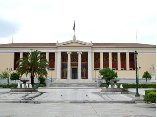
\includegraphics[width=0.9\columnwidth]{Athens_University_main_building}
	\caption{Figure captions should be placed below the figure, exactly like this. This photo shows the main building of the University of Athens.\label{fig:example}}
\end{figure}

Always refer to tables and figures in the main text, for example:
see Figure \ref{fig:example} and \tabref{tab:example}.
Figures and tables may extend across both columns to a maximum width of 17.2~cm.

Vectorial figures are preferred, e.g., eps.
When using \texttt{Matlab}, 
export using either Postscript or PDF format. 
Also, in order to optimize readability, the font size of text within a figure should be at list identical to footnote font size. If bitmap figures are used, please make sure that the resolution is enough for print quality. 
%\begin{figure}[t]
%\figbox{
%\subfloat[][]{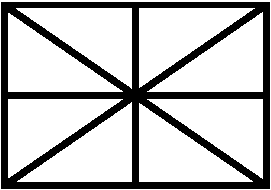
\includegraphics[width=60mm]{figure}\label{fig:subfigex_a}}\\
%\subfloat[][]{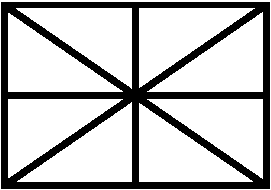
\includegraphics[width=80mm]{figure}\label{fig:subfigex_b}}
%}
%\caption{Here's an example using the subfig package.\label{fig:subfigex} }
%\end{figure}

\subsection{Footnotes}
Indicate footnotes with a number in the text \footnote{This is a footnote.}.
Use 8~pt size for footnotes. Place the footnotes at the bottom of the page 
on which they appear. 
Precede the footnote with a 0.5~pt horizontal rule.

\newpage

\section{Citations}
All bibliographical references should be listed at the end, inside a section named ``REFERENCES''.

References must be numbered in order of appearance. Please avoid listing references that do not appear in the text.

Reference numbers in the text should appear within square brackets, such as 
in~\cite{Someone:13} or~\cite{Someone:04,Someone:09}.

The reference format is the standard IEEE one. We recommend using BibTeX to create the reference list.


\section{Conclusions}
Please, submit full-length papers. Submission is fully electronic and automated through the Conference Management System. 
\underline{Do not} send papers directly by e-mail.

\begin{acknowledgments}
At the end of the Conclusions, acknowledgements to people, projects, funding agencies, etc. can be included after the second-level heading ``Acknowledgments'' (with no numbering).
\end{acknowledgments} 

%%%%%%%%%%%%%%%%%%%%%%%%%%%%%%%%%%%%%%%%%%%%%%%%%%%%%%%%%%%%%%%%%%%%%%%%%%%%%
%bibliography here
\bibliography{icmcsmc2014template}

\end{document}
